\chapter{Journal}\label{Journal}

\section*{Dag 1\&2. 05-01-2026/06-01-202}
\vspace{1em}

Idag har vi lavet opgave 1,2 \& 3.


\textbf{Exercise 1.1 - Getting Started with the STM32}

STM Cube Ide blev downloaded og configureret. :)

\textbf{Exercise 1.2 - Uploading Code to the STM3}

\begin{figure}[h]
    \centering
    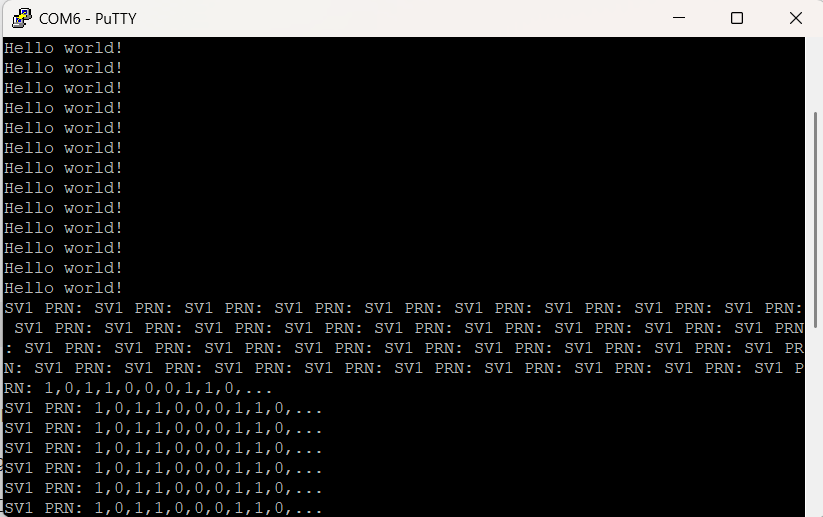
\includegraphics[width=0.75\textwidth]{Picturs/Journal/output 05-01-2026 mikrokontroller.png}
    \caption{Hello world program}
    \vspace{-2em}
\end{figure}

\vspace{1em}

\textbf{Exercise 1.3 Multiple Source Files}

\begin{figure}[h]
    \centering
    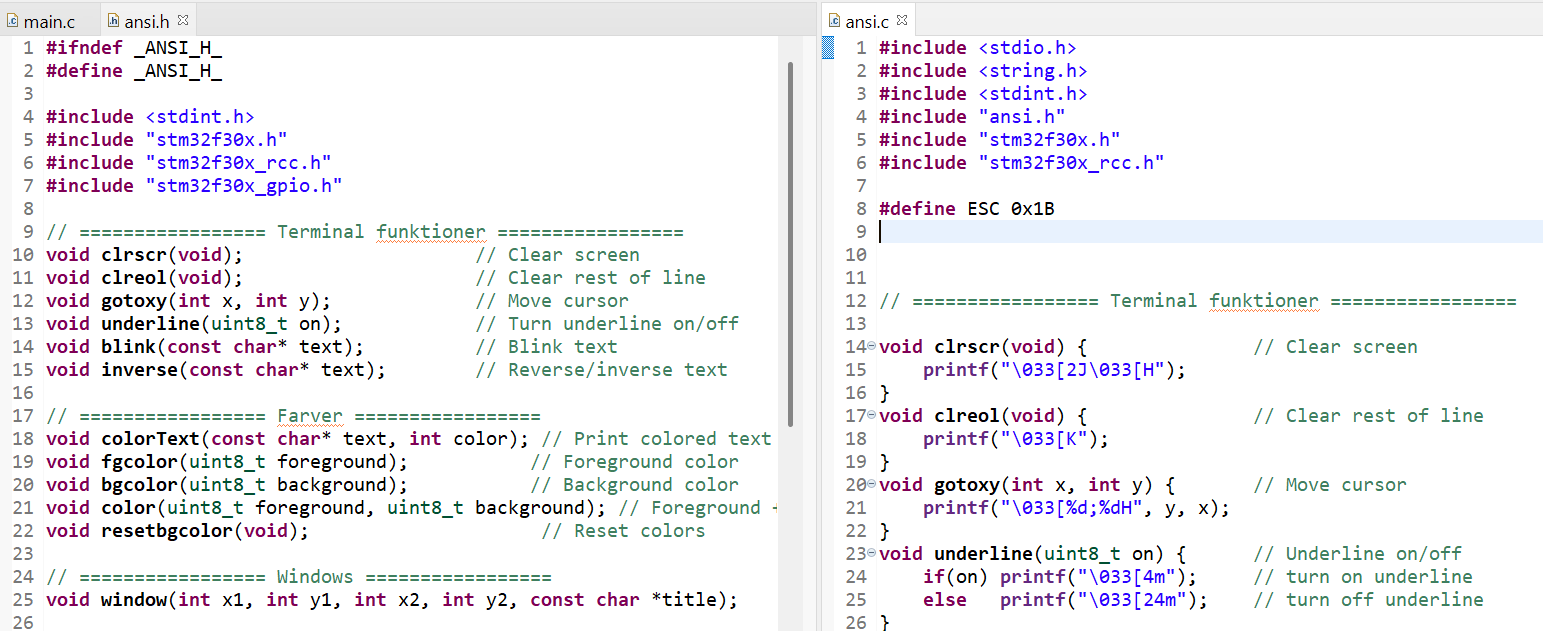
\includegraphics[width=1\textwidth]{Picturs/Journal/opgave1.3.png}
    \caption{ansi.c og ansi.h fil med funktioner}
    \vspace{-2em}
\end{figure}

\vspace{1em}

\textbf{Exercise 1.3 – Debugging}

Vejlednigen for debugging er blevet fuldt.

\vspace{1em}

\textbf{Exercise 1.4 - Integer Number Representation}

\vspace{-1em}

\begin{table}[h]
\centering
\begin{tabularx}{\textwidth}{|l|c|*{5}{>{\centering\arraybackslash}X|}}
\hline
     & Bits & Unsigned & Signed-magnitude & Ones complement & Twos complement & Biased \\ \hline
56   & 8    & 00111000 & 00111000 & 00111000 & 00111000 & 10110111 \\ \hline
178  & 16   & 00000000 10110010 & 00000000 10110010 & 00000000 10011101 & 00000000 10011110 & 10000000 10110001 \\ \hline
1002 & 16   & 00000011 11101010 & 00011101 10100010 & 00000011 11101010 & 00000011 11101010 & 10000011 11101001 \\ \hline
7586 & 16   & 00011101 10100010 & 00011101 10100010 & 00011101 10100010 & 00011101 10100010 & 10011101 10100001 \\ \hline
\end{tabularx}
\end{table}

\vspace{-2em}

\begin{table}[h]
\centering
\begin{tabularx}{\textwidth}{|l|c|*{5}{>{\centering\arraybackslash}X|}}
\hline
     & Bits & Unsigned & Signed-magnitude & Ones complement & Twos complement & Biased \\ \hline
-56  & 8    & ---      & 10111000         & 11000111        & 11001000        & 10110111 \\ \hline
-178 & 16   & ---      & 10000000 10110010 & 11111110 1001101 & 11111110 1001110 & --- \\ \hline
-1002& 16   & ---      & 10011101 10100010 & 11100010 01011101 & 11100010 01011110 & --- \\ \hline
-7586& 16   & ---      & 10011101 10100010 & 11100010 01011101 & 11100010 01011110 & --- \\ \hline
\end{tabularx}
\end{table}

\begin{lstlisting}
x = 1
y = not 0

if x==y:
    print("same")
else:
    print("Not same")
\end{lstlisting}

\vspace{-2em}

\textbf{Exercise 2.1 - ANSI Escape Codes}

\begin{lstlisting}
#ifndef ANSI_H_
#define ANSI_H_

#include <stdint.h>
#include <stdio.h>

void fgcolor(uint8_t foreground);
void bgcolor(uint8_t background);
void color(uint8_t foreground, uint8_t background);

#endif /* ANSI_H_ */
\end{lstlisting}

\vspace{-2em}

\textbf{Exercise 2.2 - Drawing Windows}
\begin{figure}[h]
    \centering
    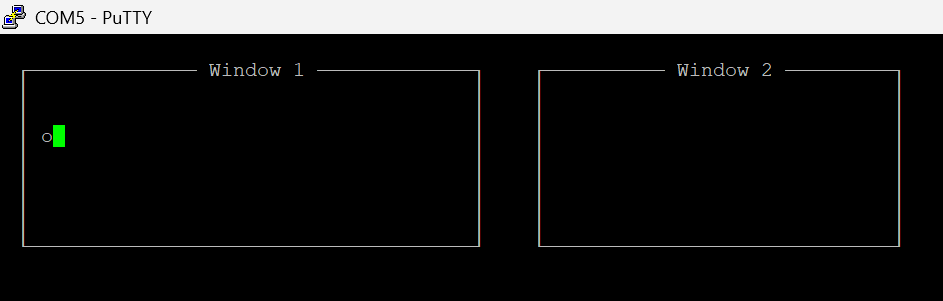
\includegraphics[width=0.82\textwidth]{Picturs/Journal/opgave2.2.png}
    \caption{Windows program}
    \vspace{-2em}
\end{figure}

\textbf{Exercise 2.3 - Bit Manipulation Question}

\keepXColumns
\begin{tabularx}{\textwidth}{|l|X|X|}
\hline
\textbf{ID} & \textbf{Spørgsmål} & \textbf{Svar} \\ \hline
\endhead

0x00 & What is 0x14 in binary? & 1=0001, 4=0100 $\rightarrow$ 14=00010100 \\ \hline
0x01 & What is 0xE6 in binary? & 11100110 \\ \hline
0x02 & What is 0x58 in binary? & 01011000 \\ \hline
0x03 & What is 10110111b in hexadecimal? & 0xB7 \\ \hline
0x04 & What is 10011111b in hexadecimal? & 0x9F \\ \hline
0x05 & What is 00111101b in hexadecimal? & 0x3D \\ \hline
0x06 & How do you turn ON bits 4 and 7 in a byte? & 0x90 (10010000) \\ \hline
0x07 & How do you turn OFF bits 2 and 5 in a byte? & 0x24 (00100100) \\ \hline
0x08 & How do you write -1 in binary, assuming size of a byte? & 10000001 (Signed-mag) / 11111111 (2's comp) \\ \hline
0x09 & How do you write -2 in binary, assuming size of a byte? & 10000010 (Signed-mag) / 11111110 (2's comp) \\ \hline
0x0A & What is 00001000b in decimal, assuming unsigned notation? & 8 \\ \hline
0x0B & What is 00001000b in decimal, assuming signed notation? & 8 \\ \hline
0x0C & What is 11111110b in decimal, assuming unsigned notation? & 254 \\ \hline
0x0D & What is 11111110b in decimal, assuming signed notation? & -2 (2's complement) \\ \hline
0x0E & What is the highest value you can store in a signed byte? & 127 (01111111) \\ \hline
0x0F & What is the highest value you can store in an unsigned byte? & 255 (11111111) \\ \hline
0x10 & What is the lowest value you can store in a signed byte? & -128 (10000000 i 2's comp) \\ \hline
0x11 & What is the lowest value you can store in an unsigned byte? & 0 (00000000) \\ \hline
0x12 & How do you tell if a signed byte is positive or negative? & Most left bit; 1 $\rightarrow$ neg, 0 $\rightarrow$ pos \\ \hline
0x13 & How do you change the sign of a binary number? & Invertér alle bits og læg 1 til (2's comp) \\ \hline
0x14 & How do you multiply a binary number by two? & Forskyd alle tal én gang til venstre ($<< 1$) \\ \hline
0x15 & How do you divide a binary number by two? & Forskyd tal til højre ($>> 1$) \\ \hline
0x16 & When dividing by two, how is rounding performed? & Ved ulige tal: Rund ned (standard shift) eller rund op ved at tilføje 1 før shift. \\ \hline
0x17 & What is the result of 0x12 | 0x01 in binary and hexadecimal? & 00010011 (0x13) \\ \hline
0x18 & What is the result of 0x13 \& 0xFE in binary and hexadecimal? & 00010010 (0x12) \\ \hline
0x19 & What is the result of $\sim$0x3F in binary and hexadecimal? & 11000000 (0xC0) \\ \hline
0x1A & What is the result of $\sim$0x01 in binary and hexadecimal? & 11111110 (0xFE) \\ \hline
0x1B & What is the result of 0x0C $>>$ 2 in binary and hexadecimal? & 00000011 (0x03) \\ \hline
0x1C & What is the result of 0x0C $>>$ 4 in binary and hexadecimal? & 00000000 (0x00) \\ \hline
0x1D & What is the result of 0x0C $<<$ 4 in binary and hexadecimal? & 11000000 (0xC0) \\ \hline
\end{tabularx}

\textbf{Exercise 3.1 – Creating a Look-up Table}

\begin{lstlisting}
#ifndef FIXED_POINT_H_
#define FIXED_POINT_H_

#include <stdint.h>

const int16_t lut[512];

void printFix(int32_t i);

int16_t sinus(int16_t);
int16_t cosinus(int16_t degree);

#endif
\end{lstlisting}

\vspace{-2em}

Declaring all of the functions and including necesarry librarie(s).

\vspace{1em}

\begin{lstlisting}
#include "fixed_point.h"

const int16_t lut[512] = {
    0, 201, 402, 603, 804, 1005, 1205,
    1406, 1606, 1806, 2005, 2205, 2404, 2603,
    2801, 2999, 3196, 3393, 3590, 3785, 3981,
    4175, 4370, 4563, 4756, 4948, 5139, 5330,
    5519, 5708, 5896, 6083, 6270, 6455, 6639,
    6822, 7005, 7186, 7366, 7545, 7723, 7900,
    8075, 8249, 8423, 8594, 8765, 8934, 9102,
    9268, 9433, 9597, 9759, 9920, 10079, 10237,
    10393, 10548, 10701, 10852, 11002, 11150, 11297,
    11441, 11585, 11726, 11865, 12003, 12139, 12273,
    12405, 12536, 12664, 12791, 12915, 13038, 13159,
    13278, 13394, 13509, 13622, 13733, 13841, 13948,
    14052, 14154, 14255, 14353, 14449, 14542, 14634,
    14723, 14810, 14895, 14977, 15058, 15136, 15212,
    15285, 15356, 15425, 15492, 15556, 15618, 15678,
    15735, 15790, 15842, 15892, 15940, 15985, 16028,
    16068, 16106, 16142, 16175, 16206, 16234, 16260,
    16283, 16304, 16323, 16339, 16352, 16363, 16372,
    16378, 16382, 16383, 16382, 16378, 16372, 16363,
    16352, 16339, 16323, 16304, 16283, 16260, 16234,
    16206, 16175, 16142, 16106, 16068, 16028, 15985,
    15940, 15892, 15842, 15790, 15735, 15678, 15618,
    15556, 15492, 15425, 15356, 15285, 15212, 15136,
    15058, 14977, 14895, 14810, 14723, 14634, 14542,
    14449, 14353, 14255, 14154, 14052, 13948, 13841,
    13733, 13622, 13509, 13394, 13278, 13159, 13038,
    12915, 12791, 12664, 12536, 12405, 12273, 12139,
    12003, 11865, 11726, 11585, 11441, 11297, 11150,
    11002, 10852, 10701, 10548, 10393, 10237, 10079,
    9920, 9759, 9597, 9433, 9268, 9102, 8934,
    8765, 8594, 8423, 8249, 8075, 7900, 7723,
    7545, 7366, 7186, 7005, 6822, 6639, 6455,
    6270, 6083, 5896, 5708, 5519, 5330, 5139,
    4948, 4756, 4563, 4370, 4175, 3981, 3785,
    3590, 3393, 3196, 2999, 2801, 2603, 2404,
    2205, 2005, 1806, 1606, 1406, 1205, 1005,
    804, 603, 402, 201, 0, -201, -402,
    -603, -804, -1005, -1205, -1406, -1606, -1806,
    -2005, -2205, -2404, -2603, -2801, -2999, -3196,
    -3393, -3590, -3785, -3981, -4175, -4370, -4563,
    -4756, -4948, -5139, -5330, -5519, -5708, -5896,
    -6083, -6270, -6455, -6639, -6822, -7005, -7186,
    -7366, -7545, -7723, -7900, -8075, -8249, -8423,
    -8594, -8765, -8934, -9102, -9268, -9433, -9597,
    -9759, -9920, -10079, -10237, -10393, -10548, -10701,
    -10852, -11002, -11150, -11297, -11441, -11585, -11726,
    -11865, -12003, -12139, -12273, -12405, -12536, -12664,
    -12791, -12915, -13038, -13159, -13278, -13394, -13509,
    -13622, -13733, -13841, -13948, -14052, -14154, -14255,
    -14353, -14449, -14542, -14634, -14723, -14810, -14895,
    -14977, -15058, -15136, -15212, -15285, -15356, -15425,
    -15492, -15556, -15618, -15678, -15735, -15790, -15842,
    -15892, -15940, -15985, -16028, -16068, -16106, -16142,
    -16175, -16206, -16234, -16260, -16283, -16304, -16323,
    -16339, -16352, -16363, -16372, -16378, -16382, -16383,
    -16382, -16378, -16372, -16363, -16352, -16339, -16323,
    -16304, -16283, -16260, -16234, -16206, -16175, -16142,
    -16106, -16068, -16028, -15985, -15940, -15892, -15842,
    -15790, -15735, -15678, -15618, -15556, -15492, -15425,
    -15356, -15285, -15212, -15136, -15058, -14977, -14895,
    -14810, -14723, -14634, -14542, -14449, -14353, -14255,
    -14154, -14052, -13948, -13841, -13733, -13622, -13509,
    -13394, -13278, -13159, -13038, -12915, -12791, -12664,
    -12536, -12405, -12273, -12139, -12003, -11865, -11726,
    -11585, -11441, -11297, -11150, -11002, -10852, -10701,
    -10548, -10393, -10237, -10079, -9920, -9759, -9597,
    -9433, -9268, -9102, -8934, -8765, -8594, -8423,
    -8249, -8075, -7900, -7723, -7545, -7366, -7186,
    -7005, -6822, -6639, -6455, -6270, -6083, -5896,
    -5708, -5519, -5330, -5139, -4948, -4756, -4563,
    -4370, -4175, -3981, -3785, -3590, -3393, -3196,
    -2999, -2801, -2603, -2404, -2205, -2005, -1806,
    -1606, -1406, -1205, -1005, -804, -603, -402,
    -201};

void printFix(int32_t i) {
// Prints a signed 16.16 fixed point number
    if ((i & 0x80000000) != 0) { // Handle negative numbers
        printf("-");
        i = ~i + 1;
    }

    printf ("%ld .%04 ld", i >> 16 , 10000 * ( uint32_t )(i & 0 xFFFF ) >> 16) ;
    // Print a maximum of 4 decimal digits to avoid overflow
    }

    int16_t sinus ( int16_t degree ) {
    return lut [ degree %512];
    }

    int16_t cosinus ( int16_t degree ) {
    return lut [( degree +128) %512];
    }
}

\end{lstlisting}

\vspace{-1em}

Pasting in all of the LUT values as well as writing the functions: printFix, sinus, and cosinus.

\vspace{1em}

\begin{lstlisting}
# include " stm32f30x_conf .h" // STM32 config
# include " 30010 _io.h" // Input / output library for this course
# include " ansi .h"
# include " fixed_point .h"

int main ( void ){
    uart_init (9600) ;
    printFix ( sinus (124) << 2) ;
    while (1) {}
}
\end{lstlisting}

\vspace{-2em}

Including all files and returning the result

\textbf{Exercise 3.2 – Sin and Cos Functions}

\begin{lstlisting}
#include <stdio.h>
#include <math.h>
#include <stdint.h>

int rotatevector(double x, double y, double angle,
                 double *diffx, double *diffy) {
    *diffx = x * cos(angle) - y * sin(angle);
    *diffy = x * sin(angle) + y * cos(angle);
    return 0;
}

int main(void) {
    double dangle;
    double a, b;
    double spliffy, spliffx;

    scanf("%lf", &dangle);
    scanf("%lf", &a);
    scanf("%lf", &b);

    rotatevector(a, b, dangle, &spliffx, &spliffy);
    printf("%f, %f\n", spliffx, spliffy);

    return 0;
}
\end{lstlisting}

\textbf{Exercise 3.3 - Vector Rotations}

\textbf{Exercise 3.4 - Bit Manipulation Questions Continued}

\keepXColumns
\begin{tabularx}{\textwidth}{|l|X|X|}
\hline
\textbf{ID} & \textbf{Spørgsmål} & \textbf{Svar} \\ \hline
\endhead
0x1E & How do you convert a char into 8.8 notation? & Shift 8 bits til venstre ($<< 8$) eller gange med 256. \\ \hline
0x1F & How do you convert an 8.8 value into a char? & Shift 8 bits til højre ($>> 8$). \\ \hline
0x20 & What is the smallest, positive, non-zero value you can store? & 1/256 (0.00390625) \\ \hline
0x21 & What happens if you add two 8.8 values? & Læg heltal og decimaler sammen normalt. \\ \hline
0x22 & What happens if you multiply two 8.8 values? & Giver et 16.16 tal, kræver shift $>> 8$ for at vende tilbage til 8.8. \\ \hline
0x23 & What happens if you multiply an 8.8 value with a char? & Resultatet forbliver i 8.8 format. \\ \hline
0x24 & What about rounding when you convert an 8.8 value to a char? & Tilføj 0x80 ($0.5$ i 8.8) før shift $>> 8$. \\ \hline
0x25 & How do you make it round correctly? & $\pm$ 0x80 afhængigt af fortegn. \\ \hline
0x26 & What is the decimal number 0.125 in hexadecimal? & 0.2 \\ \hline
0x27 & What is the decimal number 0.25 in hexadecimal? & 0.4 \\ \hline
0x28 & What is the decimal number 2.125 in hexadecimal? & 2.2 \\ \hline
0x29 & What is the decimal number 2.25 in hexadecimal? & 2.4 \\ \hline
0x2A & What is the result of 0.125*0.25 using fixed point? & 0,03125 \\ \hline
0x2B & What is the result of 2.125*2.25 using fixed point? & 4,78125 \\ \hline
0x2C & What goes wrong in question (0x2B)? & Overflow kan forekomme hvis resultatet overstiger 8.8. \\ \hline
0x2D & How can the issue of (0x2B) be addressed? & Brug en større variabel (f.eks. 16.16) til mellemregningen. \\ \hline
\end{tabularx}
